\documentclass[oneside]{scrbook}

% Font-/Inputencoding.
\usepackage[T1]{fontenc}
\usepackage[utf8]{inputenc}

% Information for PDF file.
\usepackage{hyperref}
\hypersetup{
  pdfauthor={Paul Jungeblut},
  pdftitle={Text Indexing, Script/Summary},
  pdfsubject={Text Indexing, Script/Summary},
  pdfkeywords={Text Indexing, Lecture Notes, Script, Summary}
}

% Colors.
\usepackage{color}

% Separations in enumerations.
\usepackage{enumitem}
\setlist{itemsep=1pt,topsep=3pt}

% Use french spacing, even though its wrong for english sentences.
\frenchspacing

% Math.
\usepackage{amsmath}
\usepackage{mathtools}
\usepackage[standard,thmmarks]{ntheorem}
\usepackage{amssymb}
\theoremstyle{break}
\theorembodyfont{\normalfont}
\renewtheorem{Definition}{Definition}[chapter]
\renewtheorem{Example}[Definition]{Example}
\theorembodyfont{\itshape}
\renewtheorem{Theorem}[Definition]{Theorem}
\renewtheorem{Lemma}[Definition]{Lemma}

% Pseudocode.
\usepackage{algorithm}
\usepackage{clrscode3e}

% Nice table lines and page wide tables.
\usepackage{tabularx}
\usepackage{booktabs}

% Disable indentation of new paragraphs.
\usepackage{parskip}

% TikZ.
\usepackage{float}
\usepackage{tikz}
\usetikzlibrary{shapes.multipart}
\usetikzlibrary{calc}

% Bibliography.
\usepackage[style=numeric, backend=biber]{biblatex}
\addbibresource{references.bib}

% Index.
\usepackage{makeidx}
\makeindex

% Layout for introducing terms.
% Parameter 1: The term to print.
% Parameter 2: The term to put into the index.
\newcommand{\defi}[2]{\emph{\textcolor{blue}{#1}}\index{#2}}

% Oneliner to embed TikZ images.
% Parameter 1: Path to the image.
% Parameter 2: Caption.
% Parameter 3: The name of the label ("fig:" will be added as a prefix).
\newcommand{\drawing}[3]{
  \begin{figure}[htbp]
    \centering
    \input{#1}
    \caption{#2}
    \label{fig:#3}
  \end{figure}
}

\begin{document}
  \pagenumbering{roman}
  \tableofcontents
  \newpage
  \pagenumbering{arabic}
  \chapter{Basic Datastructures}

\begin{Definition}
  Let $\Sigma = \{0, \ldots, \sigma - 1\}$ be a finite, ordered set. The elements of $\Sigma$ are called \defi{characters}{Character} or \defi{symbols}{Symbol} and $\Sigma$ is called an \defi{alphabet}{Alphabet} of size $\sigma$.
\end{Definition}

\begin{Definition}
  A \defi{string}{String} $S$ is a sequence of characters from an alphabet $\Sigma$.
  \begin{itemize}
    \item We usually use $n = \vert S \vert$ to be the length of the string.
    \item The $i$-th character of $S$ is $S[i]$. Indices are $0$-based.
    \item The substring from the $i$-th to the $j$-th character is $S[i..j]$.
    \item A substring with $i = 0$ is called \defi{prefix}{Prefix}. A substring with $j = n - 1$ is called \defi{suffix}{Suffix}.
    \item The $i$-th suffix is $S[i..n-1]$.
  \end{itemize}
\end{Definition}

\section{Suffix Tries}

\begin{Definition}
  Let $S = \{S_0, S_1, \ldots, S_{N-1}\}$ be a set of strings over an alphabet $\Sigma$. A \defi{trie}{Trie} $\mathcal{T}$ is a tree, where each node represents a different prefix in the set $S$. The root represents the empty prefix $\varepsilon$. Vertex $u$ representing prefix $Y$ is a child of vertex $v$ representing prefix $X$, if and only if $Y = Xc$ for some character $c \in \Sigma$. The edge $(v,u)$ is then labeled $c$.\\
  If $S$ is the set of all suffixes of a string $T$, the trie is called \defi{suffix trie}{Suffix Trie}.
\end{Definition}

\begin{Example}
  Figure~\ref{fig:suffixTrieExample} shows the suffix trie for the string "banana\$". The dollar sign "\$" is a sentinel that does not appear elsewhere in the text. This guarantees, that no suffix is a prefix of another suffix and the suffix trie therefore has $n+1$ leaves.
  \drawing{basicDatastructures/tikz/suffixTrieExample.tex}{The suffix trie for the string "banana\$"}{suffixTrieExample}
\end{Example}

To construct a trie over string set $S = \{S_0, \ldots, S_{N-1}\}$, we need $\mathcal{O}(\vert S_0 \vert + \ldots + \vert S_{N-1} \vert)$ steps. This bound is tight: If all characters are pairwise distinct in all strings and no two strings share a character, than the number of different prefixes and therefore vertices is given by $1 + \sum_{i=0}^{N-1} \vert S_i \vert$, where the additional $1$ represents the empty prefix $\varepsilon$.\\
The time needed to search for a string $T$ of length $m = \vert T \vert$ in the trie depends on the implementation of the tree. If the children of each vertex are stored in a list, the time is in $\mathcal{O}(m\sigma)$. If the children are stored in a sorted array (using the order of the characters in the alphabet), the time is in $\mathcal{O}(m\log \sigma)$. By using a hash table and perfect hashing, the time is in $\mathcal{O}(m)$.

The space needed to store the suffix trie $\mathcal{T}$ for a string of length $n$ is in $\mathcal{O}{(n^2\log \sigma + n^2\log n)}$ bits. The first summand is the space needed to store the $\mathcal{O}(n^2)$ edge labels of one character $c \in \Sigma$ each. The second summand is the space needed to store the pointers to the children of each node.


\section{Suffix Trees}

\begin{Definition}
  A \defi{suffix tree}{Suffix Tree} $\mathcal{T}$ for a string $S$ is the suffix trie of $S$ where each unary path is converted into a single edge. Those edges are labeled with the concatenation of the characters from the replaced edges. The leaves of the suffix tree store the text position where the corresponding suffix starts.
\end{Definition}

\begin{Example}
  Figure~\ref{fig:suffixTreeExample} shows the suffix tree for the string "banana\$". It contains only $11$ vertices compared to the $23$ vertices of the suffix trie.
  \drawing{basicDatastructures/tikz/suffixTreeExample.tex}{The suffix tree for the string "banana\$".}{suffixTreeExample}
\end{Example}

The suffix array can be constructed in time $\mathcal{O}(n)$ with algorithms by \textsc{Weiner}\cite{Weiner1973}, \textsc{McCreight}\cite{McCreight1976} or \textsc{Ukkonen}\cite{Ukkonen1995}. It needs $\mathcal{O}(n\log n + n\log \sigma)$ bits. The first summand is the space needed for the pointers to the children and the indices stored in the leaves. The second summand is the space needed for the edge labels. To achieve this space, the edge labels must not be stored explicitly. Instead we can store pointers to the first and last position of the label in the text.

In practice, a suffix tree needs more than $20$ times the space of the original text. Based on the required functionality, this can even be worse.

\section{Bitvectors}

\begin{Definition}
  A \defi{bitvector}{Bitvector} $B$ is an array of bits that are compactly stored. A bitvector supports the following operations:
  \begin{itemize}
    \item $\proc{Access}(i)$ returns the $i$-th element in $B$.
    \item $\proc{Rank}_q(i)$ returns the number of $q$-bits in the prefix $[0..i-1]$ of $B$. If $q$ is omitted, we assume $q = 1$.
    \item $\proc{Select}_q(i)$ returns the position of the $i$-th $q$-bit. If $q$ is omitted, we assume $q = 1$.
  \end{itemize}
\end{Definition}

\begin{Theorem}
  \label{thm:bitvectorRank}
  The $\proc{Rank}$-Operation on bitvectors can be done constant time and $o(n)$ additional space.\cite{Jacobson1989}
\end{Theorem}

\begin{Proof}
  Let $B$ be a bitvector of length $n$. Precompute the following information:
  \begin{enumerate}
    \item Divide $B$ into \emph{superblocks} $SB_1, \ldots, SB_{\lceil \frac{n}{L} \rceil}$ of size $L$.
    \item For each superblock $SB_j$ now store $\sum_{i=0}^{(j-1)L-1} B[i]$. This is the number of set bits in the first $j$ superblocks. For each superblock this needs $\mathcal{O}(\log n)$ bits of space.
    \item Now further divide each superblock $B_j$ into blocks $B_1^j, \ldots, B_{\lceil \frac{L}{S} \rceil}^j$ of size $S$.
    \item For each block $B_k^j$ of superblock $SB_j$ store $\sum_{i=(j-1)L}^{(j-1)L+kS-1} B[i]$. This is the number of set bits in the first $k$ blocks of superblock $SB_j$. For each block this needs $\mathcal{O}(\log L)$ bits.
  \end{enumerate}
  For a given $\proc{Rank}(i)$ query we now calculate the corresponding superblock $SB_j$ and block $B_k$. We use the precomputed sums to get the number of set bits in all superblocks before $SB_j$ and all blocks before $B_k$. All thats missing now is the number of set bits in block $B_k$ until position $i$. If the blocks are small enough, this information can be precomputed efficiently for all possible blocks and positions (Four-Russians-Trick).

  We still need to choose $L$ and $S$:
  \begin{align}
    L &= \log^2 n \\
    S &= \frac{1}{2} \log n
  \end{align}

  Let's look at the space needed:
  \begin{itemize}
    \item Prefix sums among the superblocks:
    \begin{align}
      \begin{aligned}
        \mathcal{O}\left(\frac{n}{L}\log n\right)
        &= \mathcal{O}\left(\frac{n}{\log^2 n}\log n\right)\\
        &= \mathcal{O}\left(\frac{n}{\log n}\right)
      \end{aligned}
    \end{align}
    \item Prefix sums among the blocks:
    \begin{align}
      \begin{aligned}
        \mathcal{O}\left(\frac{n}{S}\log L\right)
        &= \mathcal{O}\left(\frac{n}{\log n}\log\log^2 n\right) \\
        &= \mathcal{O}\left(\frac{n}{\log n} \cdot \log\log n\right) \\
        &= \mathcal{O}\left(\frac{n \log\log n}{\log n}\right)
      \end{aligned}
    \end{align}
    \item The lookup tables for each block. There are $2^S$ possible blocks and for each of them we need to store $S$ prefix sums in $\mathcal{O}(\log S)$ bits:
    \begin{align}
      \begin{aligned}
        \mathcal{O}\left(2^S \cdot S \cdot \log S\right)
        &= \mathcal{O}\left(2^{\frac{1}{2}\log n} \cdot \frac{1}{2}\log n \cdot \log \frac{1}{2}\log n\right) \\
        &= \mathcal{O}\left(\sqrt{n}\log n \log\log n\right)
      \end{aligned}
    \end{align}
  \end{itemize}

  The total amount of space needed is therefore $\mathcal{O}\left(\frac{n}{\log n} + \frac{n\log\log n}{\log n} + \sqrt{n}\log n\log\log n\right) = o(n)$ bits.
\end{Proof}

\section{Compressed Bitvector}

\begin{Definition}
  \label{def:zerothOrderEntropy}
  Given a sequence $X$ of length $n$ over an alphabet $\Sigma$. Let $n_c$ be the number of occurrences of character $c \in \Sigma$ in $X$.
  \begin{align}
    \mathcal{H}_0(X) := \sum\limits_{\substack{c \in \Sigma\\ n_c > 0}} \frac{n_c}{n}\log\frac{n}{n_c}
  \end{align}
  is called the \defi{zeroth order empirical entropy}{$\mathcal{H}_0$} and provides lower bound for the number of bits needed to compress $X$ using a compressor which just considers character frequencies.
\end{Definition}

\subsection{Elias-Fano Encoded Bitvector}

\begin{Theorem}
  \label{thm:eliasFanoEncoding}
  Given a non-decreasing sequence $X$ of length $m$ over the alphabet $[0,n]$. Sequence $X$ can be compressed using $2m + m\log\frac{n}{m} + o(m)$ bits while each element can still be accessed in constant time. This is known as \defi{Elias-Fano-Encoding}{Elias-Fano-Encoding}.
\end{Theorem}

\begin{Proof}
  Divide each element into a high-part and a low-part: The first $\lfloor \log m \rfloor$ bits correspond to the high-part, the other $\lceil \log n \rceil - \lfloor \log m \rfloor$ bits correspond to the low-part. The sequence of high-parts of $X$ is also non-decreasing. We use a unary gap encoding to represent the gaps and store the result in a bitvector $H$. For a gap of size $\delta_i$ we use $\delta_i + 1$ bits ($\delta_i$ zeros and $1$ one). The sum of the gaps (the total number of zeros in $H$) is at most $2^{\lfloor \log m \rfloor} \leq 2^{\log m} = m$. Therefore $H$ has size at most $2m$ (\#zeros + \#ones). The low parts can be stored explicitly.

  \begin{algorithm}[htb]
    \begin{codebox}
      \Procname{$\proc{Elias-Fano-Access}(i)$}
      \li $p \gets \proc{Select}_1(i + 1, H)$
      \li $x \gets p - i$
      \li \Return  $x \cdot 2^{\lceil\log n\rceil - \lfloor\log m\rfloor} + L[i]$
    \end{codebox}
    \caption{Access to the $i$-th element of \id{X}.}
    \label{alg:eliasFanoAccess}
  \end{algorithm}

  Algorithm~\ref{alg:eliasFanoAccess} provides a method to access the $i$-th element of the sequence in constant time.
\end{Proof}

Theorem~\ref{thm:eliasFanoEncoding} can be used to compress a bitvector~$B$. Let~$n$ be the length of~$B$ and~$m$ be the number of set bits. Further let $X$ be the positions of the set bits. $X$ forms an increasing sequence and therefore be used for compression.

\begin{Example}
  \begin{table}[htbp]
    \centering
    \begin{tabular}{ccccccccc}
      \toprule
      $X$ & $=$ & $4$ & $13$ & $15$ & $24$ & $26$ & $27$ & $29$ \\
      \midrule
      & &
      \texttt{00|100} &
      \texttt{01|101} &
      \texttt{01|111} &
      \texttt{11|000} &
      \texttt{11|010} &
      \texttt{11|011} &
      \texttt{11|101} \\

      $\delta$ & $=$ & $0$ & $1$ & $0$ & $2$ & $0$ & $0$ & $0$ \\
      $H$ & $=$ & \multicolumn{7}{l}{\texttt{1011001111}} \\
      $L$ & $=$ & \multicolumn{7}{l}{\texttt{4, 5, 7, 0, 2, 3, 5}} \\
      \bottomrule
    \end{tabular}
    \caption{Elias-Fano-Encoding for a given sequence $X$.}
    \label{tbl:eliasFanoExample}
  \end{table}
  Table~\ref{tbl:eliasFanoExample} shows how the bitvector $B=(4,13,15,24,26,27,29)$ gets encoded. The length of $B$ is $7$, so $\lfloor \log 7 \rfloor = 2$ are in the high-part and $\lceil \log 29 \rceil - \lfloor \log 7 \rfloor = 3$ bits are in the low-part. The second row shows the binary representation of each elements, the vertical bar separates the low- and the high-part. Line $\delta$ shows the differences between two consecutive high-parts. Lines $H$ and $L$ now show the compressed high-parts and the explicitly stored low-parts.
\end{Example}

\subsection{$\mathcal{H}_0$-Compressed Bitvector}

Let $B$ be a bitvector of length $n$ with $\kappa$ bits set. The entropy of this bitvector is
\begin{align}
  \mathcal{H}_0(B) = \frac{\kappa}{n}\log\frac{n}{\kappa} + \frac{n-\kappa}{n}\log\frac{n}{n - \kappa}
  \text{.}
\end{align}

\begin{Theorem}
  A bitvector can be represented in $n\mathcal{H}_0(B) + o(n)$ bits space while \proc{Rank} and \proc{Select} queries can be executed in constant time.
\end{Theorem}

\begin{Proof}
  Split the bitvector into blocks of length $K = \frac{1}{2}\log n$ bits. For each block $i$ we store the number of set bits $\kappa_i$ using $\lceil \log K + 1\rceil$ bits. These identifiers sum up to $\mathcal{O}(n\frac{\log\log n}{\log n})$ bits.

  Now we represent each block as a tuple $(\kappa_i,r_i)$. The first element $0 \leq \kappa_i \leq K$ is the number of set bits in this block. The second element $0 \leq r_i < \binom{K}{\kappa_i}$ is the index within the class.
  \begin{align}
    \begin{aligned}
      \vert B \vert
      &= \sum\limits_{i=0}^\frac{n-1}{K} \left\lceil\log\binom{K}{\kappa_i}\right\rceil \\
      &\leq \log\left(\prod\limits_{i=0}^{\frac{n-1}{K}}\binom{K}{\kappa_i}\right) + \left\lceil\frac{n}{K}\right\rceil \\
      &\leq \log\binom{n}{\kappa_0 + \ldots + \kappa_{(n-1)/K}} + \left\lceil\frac{n}{K}\right\rceil \\
      &= \log\binom{n}{K}  + \left\lceil\frac{n}{K}\right\rceil\\
      &\leq n\mathcal{H}_0(B) + \left\lceil\frac{n}{K}\right\rceil \\
      &= n\mathcal{H}_0(B) + \mathcal{O}\left(\frac{n}{\log n}\right)
    \end{aligned}
  \end{align}
  In total this gives a space requirement of $n\mathcal{H}_0(B) + \mathcal{O}\left(\frac{n}{\log n}\right) + \mathcal{O}(n\frac{\log\log n}{\log n}) = n\mathcal{H}_0(B) + o(n)$ bits. We will not go into the implementation of \proc{Rank} and \proc{Select} here.
\end{Proof}

To encode and decode a block with $\kappa$ bits set we must be able to transform the bitstring into the $(\kappa, r)$ pair and vice versa. We can do this on-the-fly by using a \defi{combinatorial number system}{Combinatorial Number System}. The idea is to give them consecutive numbers from $0$ to $\binom{K}{\kappa}-1$ in the order given by their values interpreted as binary numbers.

% TODO (pjungeblut): This can nicely be visualised.
\begin{itemize}
  \item To encode a given bitstring initialize $r = 0$ and go through the bits from left to right. If the first bit is a $0$, we just drop it, decrement $K$ and continue with the remaining bits. If the first bit is a $1$, we know that there is $\binom{K-1}{\kappa-1}$ other possible bitstrings that start with $0$ and contain $\kappa$ bits. Therefore we increase $r$ by $\binom{K-1}{\kappa-1}$, decrement $K$ and $\kappa$ and continue with the next bit.
  \item To decode a given pair $(\kappa, r)$, we check if $r \geq \binom{K}{\kappa}$. If so, the first bit is a $1$ and we subtract $\binom{K}{\kappa}$ from $r$, decrease $K$ and $\kappa$ and continue to get the next bit. If $r < \binom{K}{\kappa}$, then the first bit is $0$ and we decrease $K$ and continue to get the next bit.
\end{itemize}

\section{Wavelet Trees}

\begin{Definition}
  A \defi{wavelet tree}{Wavelet Tree} is a compact datastructure that stores a sequence $S$ and generalizes the operations of a bitvector to an arbitrary alphabet.
  \begin{itemize}
    \item $\proc{Access}(i)$ returns the $i$-th element of the sequence.
    \item $\proc{Rank}_q(i)$ returns the number of occurrences of $q$ in the prefix $S[0..i-1]$.
    \item $\proc{Select}_q(i)$ returns the position of the $i$-th occurrence of $q$ in $S$.
  \end{itemize}

  The root of the wavelet tree stores the whole sequence. Each vertex recursively divides its sequence to its two children. The left child contains the first half of the remaining alphabet, the right child contains the second half of the remaining alphabet. A bitvector in every vertex stores the corresponding child for each element.
\end{Definition}

\begin{Lemma}
  A wavelet tree can be stored in $n\lceil\log\sigma\rceil$ bits space.
\end{Lemma}

\begin{Proof}
  The wavelet tree has height $\lceil\log\sigma\rceil$ and stores $n$ bits on every layer (maybe even less on the last layer). Therefore $n\lceil\log\sigma\rceil$ bits are needed to store the bitvectors. A wavelet tree can be implemented fully via bitvectors and does not need any pointers. This will be demonstrated in more detail below.
\end{Proof}

\begin{Example}
  \label{exp:waveletTree}
  Figure~\ref{fig:waveletTreeExample} shows the wavelet tree for the string "abracadabra". By concatenating the bitvectors in each vertex in level order from left to right, we fully describe the wavelet tree. The bitvector describing this wavelet tree is \texttt{00100010010|00010000|101|0100010}, where the vertical lines show the borders between consecutive vertices. They do not need to be stored, because all layers (except maybe the last layer) contain exactly $n$ bits.
  \drawing{basicDatastructures/tikz/waveletTreeExample.tex}{The wavelet tree for the string "abracadabra".}{waveletTreeExample}
\end{Example}

When storing the wavelet tree in a single bitvector $B$ as in Example~\ref{exp:waveletTree}, each vertex can be described by two indices giving the position of the bitvector of the vertex in $B$. For example the root corresponds to the pair $[0,n-1]$. Algorithm~\ref{alg:waveletTreeLevel} shows how to get the level of a vertex $v$ of the wavelet tree. This just uses the fact, that every level contains $n$ bits. Algorithm~\ref{alg:waveletTreeSize} just calculates the length of the string stored in the given vertex. Algorithm~\ref{alg:waveletTreeLeftChild} and Algorithm~\ref{alg:waveletTreeRightChild} return the indices for the left and the right child of the given vertex. Assuming that we can execute the rank queries in constant time (Theorem~\ref{thm:bitvectorRank}), they both run in constant time. It is also possible to implement a \proc{Parent}-function, but this needs additional information, such as whether the current vertex is a left or a right child of its parent.

\begin{algorithm}[htb]
  \begin{codebox}
    \Procname{$\proc{Level}(v=[l,r])$}
    \li \Return $\left\lceil \frac{l}{n} \right\rceil$
  \end{codebox}
  \caption{Returns the level of a vertex of the wavelet tree.}
  \label{alg:waveletTreeLevel}
\end{algorithm}

\begin{algorithm}[htb]
  \begin{codebox}
    \Procname{$\proc{Size}(v=[l,r])$}
    \li \Return $r - l + 1$
  \end{codebox}
  \caption{Returns the number of elements stored in a vertex of the wavelet tree.}
  \label{alg:waveletTreeSize}
\end{algorithm}

\begin{algorithm}[htb]
  \begin{codebox}
    \Procname{$\proc{Left-Child}(v=[l,r])$}
    \li $l' \gets l + n$
    \li $r' \gets l' + \proc{Size}(v) - (\proc{Rank}(r + 1) - \proc{Rank}(l)) - 1$
    \li \Return $[l',r']$
  \end{codebox}
  \caption{Returns the left child of a vertex of the wavelet tree.}
  \label{alg:waveletTreeLeftChild}
\end{algorithm}

\begin{algorithm}[htb]
  \begin{codebox}
    \Procname{$\proc{Right-Child}(v=[l,r])$}
    \li $r' \gets r + n$
    \li $l' \gets r' - (\proc{Rank}(r + 1) - \proc{Rank}(l) - 1)$
    \li \Return $[l',r']$
  \end{codebox}
  \caption{Returns the right child of a vertex of the wavelet tree.}
  \label{alg:waveletTreeRightChild}
\end{algorithm}

\begin{Theorem}
  \label{thm:waveletTreeAceess}
  The $\proc{Access}(i)$-operation can be implemented in $\mathcal{O}(\log \sigma)$.
\end{Theorem}

\begin{Proof}
  To access the $i$-th element we check the $i$-th position in the root-bitvector. If it is $0$, the element is stored in the left child and the new index there is $i - \proc{Rank}(i)$. If it is $1$, the element is in the right child and the new index there is $i - \proc{Rank}_0(i)$, where $\proc{Rank}_0(i) := i - \proc{Rank}(i)$ is the number of $0$-bits before position $i$.

  This can be done in $\mathcal{O}(\log\sigma)$, because the wavelet tree has a height of $\log\sigma$ and the rank queries can be done in constant time on bitvectors.
\end{Proof}

\begin{Theorem}
  \label{thm:waveletTreeRank}
  The $\proc{Rank}_q(i)$-operation can be implemented in $\mathcal{O}(\log \sigma)$.
\end{Theorem}

\begin{Proof}
  $\proc{Rank}_q(i)$-queries can be answered the same way as $\proc{Access}(i)$-queries. The $\proc{Access}(i)$-query descents into the leaf containing all $q$ symbols with some modified index $i'$. The rank is the number of elements before $i'$, so $i'-1$. Since no additional work needs to be done, the runtime is in $\mathcal{O}(\log\sigma)$.
\end{Proof}

\begin{Theorem}
  \label{thm:waveletTreeSelect}
  The $\proc{Select}_q(i)$-operation can be implemented in $\mathcal{O}(\log \sigma)$.
\end{Theorem}

\begin{Proof}
  % TODO (pjungeblut): This uses the fact, that select-queries can be done in
  %                    constant time on bitvectors. This is not yet proven in
  %                    this document. If added, also remove parentheses from
  %                    the last sentence in the following paragraph.
  For a $\proc{Select}_q(i)$-query we start in the leave corresponding to symbol $q$ at position $i$. This can be found the same way as in the $\proc{Access}$-operation. Now we recursively process the parents until reaching the root. If the current vertex is a left child, the new position is the position of the $i$-th $0$ in the parent bitvector. If it is a right child, the new position is the position of the $i$-th $1$ in the parent bitvector. This needs $\proc{Select}$-queries on bitvectors, which can be done in constant time (not part of this document yet).
\end{Proof}

\section{$\mathcal{H}_0$-Compression for Sequences}

\begin{Definition}
  Let $S$ be a sequence of length $n$ over an alphabet $\Sigma = [0, \sigma - 1]$ of size $\sigma$. Again $n_c$ is the number of occurrences of $c \in \Sigma$ in $S$.
  \begin{align}
    \mathcal{H}_0(S) = \sum\limits_{\substack{c \in \Sigma\\ n_c > 0}} \frac{n_c}{n}\log\frac{n}{n_c}
  \end{align}
\end{Definition}

The idea to compress $S$ is to represent $S$ as a wavelet tree using $\mathcal{H}_0$-compressed bitvectors. For a bitstring $\omega$, $S_\omega$ we will denote the node in the wavelet tree containing all symbols from $S$ whose binary representations starts with $\omega$. So $S_\varepsilon$ is the root, $S_0$ the left child of it and $S_{10}$ the left child of the right child of the root.

\begin{Theorem}
  A sequence $S$ of length $n$ with alphabet $\sigma$ can be represented with a wavelet tree in space $n\mathcal{H}_0(S)$ bits.
\end{Theorem}

\begin{Proof}
  We will proof the claim by induction. Let $H$ be the height of the wavelet tree. For a leaf $S_c$ of the wavelet tree we get $\mathcal{H}_0(S_c) = 0$. Now as the induction hypothesis assume that the claim holds for all nodes $S_\omega$ where $\omega$ is a binary string of length $L$.

  Now consider a subsequence $S_\omega$ corresponding to an inner vertex, where $\omega$ is a binary string of length $L - 1$. By our induction hypothesis the space needed to represent $S_{\omega 0}$ and $S_{\omega 1}$ is $n_{\omega 0}\mathcal{H}_0(S_{\omega 0})$ and $n_{\omega 1}\mathcal{H}_0(S_{\omega 1})$. Now the space needed to encode $S_\omega$ is ($B_\omega$ is the bitvector in the node corresponding to $S_\omega$):
  \begin{align}
    \begin{aligned}
      \proc{Space}(S_\omega)
      &= n_\omega\mathcal{H}_0(B_\omega) + n_{\omega 0}\mathcal{H}_0(S_{\omega 0}) + n_{\omega 1}\mathcal{H}_0(S_{\omega 1}) \\
      &= n_{\omega 0}\log\frac{n_\omega}{n_{\omega 0}} + n_{\omega 1}\log\frac{n_\omega}{n_{\omega 1}} + n_{\omega 0}\mathcal{H}_0(S_{\omega 0}) + n_{\omega 1}\mathcal{H}_0(S_{\omega 1}) \\
      &= \underbrace{n_{\omega 0}\log\frac{n_\omega}{n_{\omega 0}} + n_{\omega 0}\mathcal{H}_0(S_{\omega 0})}_{(a)} + \underbrace{n_{\omega 1}\log\frac{n_\omega}{n_{\omega 1}} + n_{\omega 1}\mathcal{H}_0(S_{\omega 1})}_{(b)} = (*)
    \end{aligned}
  \end{align}
  For $(a)$ (and analogously $(b)$) we can now substitute the definition of $n_{\omega 0}\mathcal{H}_0(S_{\omega 0}) = \sum_{\alpha \in \sigma^{H - L}} n_{\omega 0\alpha} \log\frac{n_{\omega 0}}{n_{\omega 0\alpha}}$. In this sum, $\alpha$ are all possible ways to extend $\omega 0$ to a prefix corresponding to a vertex in the wavelet tree. We get:
  \begin{align}
    \begin{aligned}
      (a)
      &= n_{\omega 0}\log\frac{n_\omega}{n_{\omega 0}} + \sum\limits_{\alpha \in \sigma^{H - L}} n_{\omega 0\alpha} \log\frac{n_{\omega 0}}{n_{\omega 0\alpha}} \\
      &= \sum\limits_{\alpha \in \sigma^{H - L}} n_{\omega 0\alpha} \log\frac{n_\omega}{n_{\omega 0}} + \sum\limits_{\alpha \in \sigma^{H - L}} n_{\omega 0\alpha} \log\frac{n_{\omega 0}}{n_{\omega 0\alpha}} \\
      &= \sum\limits_{\alpha \in \sigma^{H - L}} n_{\omega 0\alpha} \left(\log\frac{n_\omega}{n_{\omega 0}} + \log\frac{n_\omega 0}{n_{\omega 0\alpha}}\right) \\
      &= \sum\limits_{\alpha \in \sigma^{H - L}} n_{\omega 0\alpha} \left(\log n_\omega - \log n_{\omega 0} + \log n_{\omega 0} - \log n_{\omega 0\alpha}\right) \\
      &= \sum\limits_{\alpha \in \sigma^{H - L}} n_{\omega 0\alpha} \log\frac{n_\omega}{n_{\omega 0\alpha}}
    \end{aligned}
  \end{align}
  Plugging the values of $(a)$ and $(b)$ we get
  \begin{align}
    \begin{aligned}
      (*)
      &= \sum\limits_{\alpha \in \sigma^{H - L}} n_{\omega 0\alpha} \log\frac{n_\omega}{n_{\omega 0\alpha}} + \sum\limits_{\alpha \in \sigma^{H - L}} n_{\omega 1\alpha} \log\frac{n_\omega}{n_{\omega 1\alpha}} \\
      &= \sum\limits_{\alpha' \in \sigma^{H - (L - 1)}} n_{\omega\alpha'} \log\frac{n_\omega}{n_{\omega\alpha'}} \\
      &= n_\omega\mathcal{H}_0(S_\omega)
    \end{aligned}
  \end{align}
  for the space of $S_\omega$.
\end{Proof}


  \chapter{Suffix Arrays}

\section{Suffix Array}

\begin{Definition}
  The \defi{suffix array}{Suffix Array} \id{SA} of a string $T$ gives the sorted order of all suffixes of $T$. Element $\id{SA}[i]$ stores the index of the $i$-th lexicographically smallest suffix of $T$.
\end{Definition}

\begin{Example}
  Consider the string $T=\texttt{abracadabrabarbara\$}$. Table~\ref{tbl:suffixArrayExample} shows the suffix array for~$T$. Note that the dollar sign \texttt{\$} is lexicographically smaller than any other character. This guarantees that suffixes which are a prefix of other suffixes appear first.
  \begin{table}[htbp]
    \centering
    \begin{tabular}{ccl}
      \toprule
      $i$  & $\id{SA}[i]$ & $T[\id{SA}[i]..n-1]$ \\
      \midrule
      $0$  & $18$         & \texttt{\$} \\
      $1$  & $17$         & \texttt{a\$} \\
      $2$  & $10$         & \texttt{abarbara\$} \\
      $3$  & $7$          & \texttt{abrabarbara\$} \\
      $4$  & $0$          & \texttt{abracadabrabarbara\$} \\
      $5$  & $3$          & \texttt{acadabrabarbara\$} \\
      $6$  & $5$          & \texttt{adabrabarbara\$} \\
      $7$  & $15$         & \texttt{ara\$} \\
      $8$  & $12$         & \texttt{arbara\$} \\
      $9$  & $14$         & \texttt{bara\$} \\
      $10$ & $11$         & \texttt{barbara\$} \\
      $11$ & $8$          & \texttt{brabarbara\$} \\
      $12$ & $1$          & \texttt{bracadabrabarbara\$} \\
      $13$ & $4$          & \texttt{cadabrabarbara\$} \\
      $14$ & $6$          & \texttt{dabrabarbara\$} \\
      $15$ & $16$         & \texttt{ra\$} \\
      $16$ & $9$          & \texttt{rabarbara\$} \\
      $17$ & $2$          & \texttt{racadabrabarbara\$} \\
      $18$ & $13$         & \texttt{rbara\$} \\
      \bottomrule
    \end{tabular}
    \caption{The suffix array for \texttt{abracadabrabarbara\$}.}
    \label{tbl:suffixArrayExample}
  \end{table}
\end{Example}

\begin{Theorem}
  We can search for all occurrences of a string $S$ in $T$ using the suffix array \id{SA} over $T$ in time $\mathcal{O}(m\log n)$, where $n = \vert T \vert$ and $m = \vert S \vert$. This is knows as \defi{forward search}{Forward Search}.
\end{Theorem}

\begin{Proof}
  We find the first suffix in \id{SA} greater or equal to $S$ and the first suffix in $T$ bigger than $S$. Assume these are at positions $i$ and $j$ with $i \leq j$. Then we have $j - i$ occurrences of $S$ in $T$ and the corresponding positions are stored in $\id{SA}[i], \ldots, \id{SA}[j-1]$. Both $i$ and~$j$ can be found using a binary search, since the suffix array is sorted. The binary search needs $\mathcal{O}(\log n)$ steps and each steps does a string comparison in $\mathcal{O}(m)$ time.
\end{Proof}

\begin{Example}
  Consider strings $T=\texttt{abracadabrabarbara\$}$ and $S=\texttt{bar}$. How often and where does~$S$ appear in $T$?

  Table~\ref{tbl:suffixArrayExample} shows the suffix array for $T$. By binary search we find $i = 9$ and $j = 11$. So~$T[\id{SA}[i] \twodots n-1]$ is the smallest suffix greater or equal than \texttt{bar} and $T[\id{SA}[j] \twodots n-1]$ is the smallest suffix greater than \texttt{bar}. We see that \texttt{bar} appears $j-i=11-9=2$ times. The occurrences are at positions $\id{SA}[9]=14$ and $\id{SA}[10]=11$.
\end{Example}

The suffix array itself needs $n\log n$ bits of space. But to work with it, we additionally need to store the text itself, which needs another $n\log\sigma$ bits of space. In total this results in a space of $n\log n + n\log\sigma$ bits.

\section{Burrows-Wheeler-Transformation}

\begin{Definition}
  The \defi{Burrows-Wheeler-Transformation}{Burrows-Wheeler-Transformation} \id{BWT} rearranges the characters of a string $T$ into runs of similar characters which makes it easier to compress.
  \begin{equation}
    \id{BWT}[i] := T[\id{SA}[i] - 1 \mod n]
  \end{equation}
  Intuitively, $\id{BWT}[i]$ is the character preceding the $i$-th suffix (or the last character for the zeroth suffix).
\end{Definition}

The \id{BWT} needs $n\log\sigma$ bits of space if it is stored uncompressed. The idea behind the \id{BWT} was better compression: Compressed size is $nH_k(T)$ bits, where $H_k(T)$ is the $k-th$ order entropy of the text $T$.

\begin{Example}
  Table~\ref{tbl:burrowsWheelerTransformationExample} shows the suffix array for the string \texttt{abracadabrabarbara\$} together with the Burrows-Wheeler-Transformation of it.
  \begin{table}[htb]
    \centering
    \begin{tabular}{cccl}
      \toprule
      $i$  & $\id{SA}[i]$ & $\id{BWT}[i]$ & $T[\id{SA}[i] \twodots n-1]$ \\
      \midrule
      $0$  & $18$    & \texttt{a}        & \texttt{\$} \\
      $1$  & $17$    & \texttt{r}        & \texttt{a\$} \\
      $2$  & $10$    & \texttt{r}        & \texttt{abarbara\$} \\
      $3$  & $7$     & \texttt{d}        & \texttt{abrabarbara\$} \\
      $4$  & $0$     & \texttt{\$}       & \texttt{abracadabrabarbara\$} \\
      $5$  & $3$     & \texttt{r}        & \texttt{acadabrabarbara\$} \\
      $6$  & $5$     & \texttt{c}        & \texttt{adabrabarbara\$} \\
      $7$  & $15$    & \texttt{b}        & \texttt{ara\$} \\
      $8$  & $12$    & \texttt{b}        & \texttt{arbara\$} \\
      $9$  & $14$    & \texttt{r}        & \texttt{bara\$} \\
      $10$ & $11$    & \texttt{a}        & \texttt{barbara\$} \\
      $11$ & $8$     & \texttt{a}        & \texttt{brabarbara\$} \\
      $12$ & $1$     & \texttt{a}        & \texttt{bracadabrabarbara\$} \\
      $13$ & $4$     & \texttt{a}        & \texttt{cadabrabarbara\$} \\
      $14$ & $6$     & \texttt{a}        & \texttt{dabrabarbara\$} \\
      $15$ & $16$    & \texttt{a}        & \texttt{ra\$} \\
      $16$ & $9$     & \texttt{b}        & \texttt{rabarbara\$} \\
      $17$ & $2$     & \texttt{b}        & \texttt{racadabrabarbara\$} \\
      $18$ & $13$    & \texttt{a}        & \texttt{rbara\$} \\
      \bottomrule
    \end{tabular}
    \caption{The suffix array for \texttt{abracadabrabarbara\$}.}
    \label{tbl:burrowsWheelerTransformationExample}
  \end{table}
\end{Example}

\begin{Theorem}
  We can search for all occurrences of a string $S$ in $T$ using the suffix array \id{SA} and the Burrwos-Wheeler-Transform \id{BWT} over $T$ in time $\mathcal{O}(m\log \sigma)$, where $m = \vert S \vert$. This is known as \defi{backward search}{Backward Search}.
\end{Theorem}

\begin{Proof}
  We need another array $C$ storing for each $c \in \Sigma$ the position of the first suffix in~\id{SA} starting with $c$. The numbers in $C$ are sorted the same way as the characters in~$\Sigma$. Array $C$ needs another $\sigma\log n$ bits of space.

  We search for all suffixes of $T$ starting with $S$. They form a consecutive interval in the suffix array \id{SA} of $T$. We start with the full interval $[\id{sp}_0,\id{ep}_0]=[0,n-1]$ corresponding to all suffixes of $T$ starting with the empty suffix $\varepsilon$ of $S$. In step $i$ ($1 \leq i \leq m$), we will shrink the interval to $[\id{sp}_i,\id{ep}_i]$ corresponding to all suffixes of $T$ starting with the last $i$ characters of $S$ (this is why its called backward search). The new interval $[\id{sp}_{i+1},\id{ep}_{i+1}]$ is defined as
  \begin{align}
    \id{sp}_{i+1} &= C[c] + \proc{Rank}_c(\id{sp}_i, \id{BWT})
    \label{eq:backwardSearchStartPos} \\
    \id{ep}_{i+1} &= C[c] + \proc{Rank}_c(\id{ep}_i + 1, \id{BWT}) - 1
    \label{eq:backwardSearchEndPos}
  \end{align}
  where $c$ is the $(i+1)$-th last character of $S$. Both operations can be done in $\mathcal{O}(\log\sigma)$ using a wavelet tree over the \id{BWT} array. The search needs $m$ steps, so the total runtime is in $\mathcal{O}(m\log\sigma)$.

  The interval given by $[\id{sp}_m,\id{ep}_m]$ in the suffix array corresponds to all occurrences of $S$ in $T$ and the positions are $\id{SA}[\id{sp}_m], \ldots, \id{SA}[\id{ep}_m]$.
\end{Proof}

The intuition behind Equation~\ref{eq:backwardSearchStartPos} and~\ref{eq:backwardSearchEndPos} is the following: $C[c]$ gives the start position of all suffixes in \id{SA} starting with the $(i+1)$-th character $c$ of $S$. But of course, only some continuous subsequence of them also starts with the whole last $i+1$ characters of $S$. This subsequence is calculated with the $\proc{Rank}_c$ queries: The \id{BWT} tells us, which of the suffixes in $[\id{sp}_i,\id{ep}_i]$ are preceded with $c$ (the $(i+1)$-th last character of $S$). To now calculate $\id{sp}_{i+1}$ from $i$, we need to know, how many suffixes starting with $c$ are lexicographically smaller than the $c$-preceded suffixes in $[\id{sp}_i,\id{ep}_i]$. The answer is just $\proc{Rank}_c(\id{sp}_i, \id{BWT})$ as in Equation~\ref{eq:backwardSearchStartPos}. For $\id{ep}_{i+1}$ Equation~\ref{eq:backwardSearchEndPos} additionally counts the number of suffixes of $T$ in $[\id{sp}_i,\id{ep}_i]$ preceded by $c$.

\begin{Example}
  We will again search for string $S=\texttt{bar}$ in the text $T=\texttt{abracadabrabarbara\$}$, this time using backward search. The suffix array and Burrows-Wheeler-Transformation of $T$ are given in Table~\ref{tbl:burrowsWheelerTransformationExample}.

  Array $C$ is given by the following Table~\ref{tbl:backwardSearchCExample} for text $T$.
  \begin{table}[htb]
    \centering
    \begin{tabular}{cccccc}
      \toprule
      \$ & a & b & c & d & r \\
      \midrule
      0 & 1 & 9 & 13 & 14 & 15 \\
      \bottomrule
    \end{tabular}
    \caption{$C$-array for the string \texttt{abracadabrabarbara\$}.}
    \label{tbl:backwardSearchCExample}
  \end{table}

  Initially $[\id{sp}_0,\id{ep}_0]=[0,n-1]$ is the whole set of all suffixes of $T$. They all match the empty suffix $\varepsilon$ of $S$. We will now go through the different steps of the backward search, the red part always highlights the current suffix of $S$ matched with the suffixes in \id{SA}.
  \begin{enumerate}
    \item Step 1 (\texttt{ba{\color{red}r}}):
    \begin{align*}
      \id{sp}_1 &= C[r] + \proc{Rank}_r(\id{sp}_0, \id{BWT}) \\
                &= 15 + \proc{Rank}_r(0, \id{BWT}) \\
                &= 15 + 0 = 15 \\
      \id{ep}_1 &= C[r] + \proc{Rank}_r(\id{ep}_0 + 1, \id{BWT}) - 1 \\
                &= 15 + \proc{Rank}_r(19, \id{BWT}) \\
                &= 15 + 4 - 1 = 18
    \end{align*}
    The suffixes starting with \texttt{r} start at position $C[r]=15$ in the suffix array and there is a total of four of them, so $[\id{sp}_1,\id{ep}_1]=[15,18]$.

    \item Step 2 (\texttt{b{\color{red}ar}}):
    \begin{align*}
      \id{sp}_2 &= C[a] + \proc{Rank}_a(\id{sp}_1, \id{BWT}) \\
                &= 1 + \proc{Rank}_a(15, \id{BWT}) \\
                &= 1 + 6 = 7 \\
      \id{ep}_2 &= C[a] + \proc{Rank}_a(\id{ep}_1 + 1, \id{BWT}) - 1 \\
                &= 1 + \proc{Rank}_a(19, \id{BWT}) \\
                &= 1 + 8 - 1 = 8
    \end{align*}
    Of the four suffixes starting with \texttt{r} found in step 1, two are preceded by \texttt{a} (at position $15$ and $18$ in the suffix array). Further there is $\proc{Rank}_a(15, \id{BWT})=6$ more suffixes preceded by \texttt{a} not starting with \texttt{r} that are lexicographically smaller, so the new interval becomes $[\id{sp}_2,\id{ep}_2]=[7,8]$.

    \item Step 3 (\texttt{{\color{red}bar}}):
    \begin{align*}
      \id{sp}_3 &= C[b] + \proc{Rank}_b(\id{sp}_2, \id{BWT}) \\
                &= 9 + \proc{Rank}_b(7, \id{BWT}) \\
                &= 9 + 0 = 9 \\
      \id{ep}_3 &= C[b] + \proc{Rank}_b(\id{ep}_2 + 1, \id{BWT}) - 1 \\
                &= 9 + \proc{Rank}_b(8, \id{BWT}) \\
                &= 9 + 2 - 1 = 10
    \end{align*}
    Both suffixes starting with \texttt{ar} in \id{SA} are preceded with \texttt{b} and there is no other, smaller suffixes in \id{SA} preceded by \texttt{b}, so the two suffixes starting with \texttt{bar} are given by $[\id{sp}_3,\id{ep}_3]=[9,10]$.
  \end{enumerate}
\end{Example}

\section{Self Index}

The suffix array together with the Burrows-Wheeler-Transformation allowed to count the occurrences of a pattern $S$ in a string $T$ in $\mathcal{O}(m\log\sigma)$. The original text was not needed at all. But when we want to print the actual occurrences, we need to access the text $T$ and therefore store it together with the index. We will now see, how we can code the text into the index.

\begin{Definition}
  A \defi{self index}{Self Index} is an index that allows fast pattern matching and efficient reconstruction of any substring of the original text.
\end{Definition}

\begin{Definition}
  Let $j = SA[i]$ be the starting position of the $i$-th smallest suffix. Then \defi{$LF[i]$}{LF-Mapping} is defined as the position of $(j-1) \mod n$ in the suffix array.
\end{Definition}

\begin{Theorem}
  $LF$ can be calculated from the Burrows-Wheeler-Transformation:
  \begin{align}
    LF[i] := C[BWT[i]] + \mathrm{rank}_{BWT[i]}(i, BWT)
    \label{eq:lfMapping}
  \end{align}
\end{Theorem}

\begin{Proof}
  We know that $BWT[i]$ is the character preceding the suffix at position $i$ in the suffix array. So the previous suffix must be in the continuous range of suffixes in the suffix array starting with $BWT[i]$. This range begins at index $C[BWT[i]]$. Then $\mathrm{rank}_{BWT[i]}(i, BWT)$ calculates the offset in this range by just counting how many suffixes also start with $BWT[i]$ and are lexicographically smaller.
\end{Proof}

\begin{Theorem}
  \label{thm:lfMapping}
  The Burrows-Wheeler-Transformation and the $LF$-array are enough information to decode the whole text $T$.
\end{Theorem}

\begin{Proof}
  We will proof this by induction.

  \textbf{Base:} We know that the last suffix is the dollar sign "\$" and that it is stored at index $0$ in the suffix array $SA$, because \$ is lexicographically smaller than all other characters of our alphabet.

  \textbf{Step:} Assume we know some character $c$ and the index $i$, where the suffix of our text starting at $c$ is in the suffix array. Then the Burrows-Wheeler-Transformation $BWT[i]$ already gives us the character preceding $c$. To be able to pull of the same trick again, we still need the position of the suffix preceding the one starting at $c$. This is just how $LF[i]$ was defined.
\end{Proof}

\begin{Definition}
  The \defi{$F$-array}{$F$-Array} contains the first characters of each suffix of text $T$ in the order they appear in the suffix array.
  \begin{align}
    F[i] := T[SA[i]]
  \end{align}
\end{Definition}

\begin{Definition}
  The inverse of $LF$ is called \defi{$\Psi$}{$\Psi$-Mapping} and maps $j = SA[i]$, the position of the $i$-th smallest suffix, to the position of $(j+1) \mod n$ in the suffix array.
\end{Definition}

\begin{Theorem}
  For a text $T$ we get
  \begin{align}
    \Psi[i] := \mathrm{select}_{F[i]}(\mathrm{rank}_{F[i]}(i, F), BWT)
    \text{.}
  \end{align}
\end{Theorem}

\begin{Proof}
  If $j = SA[i]$ is the position of the $i$-th lexicographically smallest suffix, then the suffix starting at position $j+1$ is preceded by $F[i]$. Therefore we know the Burrows-Wheeler-Transformation $BWT[\Psi[i]] = F[i]$. This is why we can calculate $\Psi$ by a $\mathrm{select}$-query on the $BWT$-array. The inner query $\mathrm{rank}_{F[i]}(i, F)$ determines which occurrence of $F[i]$ in the $BWT$-array we are interested in. If the suffix at position $i$ in the suffix array is the $k$-th smallest starting with $F[i]$, then we look for the $k$-th occurrence of $F[i]$ in the $BWT$-array.
\end{Proof}

Function $\Psi$ allows to reconstruct the text from the front in contrast to $LF$, which can reconstruct it from the back as described in Theorem~\ref{thm:lfMapping}.

\begin{Definition}
  The suffix array is a permutation of the integers in $[0,n]$. The inverse permutation $ISA$ is called the \defi{inverse suffix array}{Inverse Suffix Array}. We get $i = ISA[SA[i]]$.
\end{Definition}

\begin{Theorem}
  \label{thm:lfPsiViaSAISA}
  $LF$ and $\Psi$ can be expressed using only the suffix array $SA$ and the inverse suffix array~$ISA$.
  \begin{align}
    LF[i] &= ISA[(SA[i] - 1) \mod n] \\
    \Psi[i] &= ISA[(SA[i] + 1) \mod n]
  \end{align}
\end{Theorem}

\begin{Proof}
  $LF[i]$ was defined as the position of $(SA[i] - 1) \mod n$ in the suffix array. If we know the inverse permutation of the suffix array $ISA$, we can just look into it for the position we want. For $\Psi$ this works analogously.
\end{Proof}

\begin{Theorem}
  $SA$, $ISA$, $LF$ and $\Psi$ can be accessed using $n \log n + o(n \log n)$ bits space each in time $\mathcal{O}(\log n)$ .
\end{Theorem}

\begin{Proof}
  We can build a wavelet tree over the suffix array $SA$. By Theorem~\ref{thm:waveletTreeAceess} we can than access each element in the suffix array in time $\mathcal{O}(\log n)$. To access the inverse suffix array $ISA$ we would need the position of some value $i$ in the suffix array. This can be done with a single $\mathrm{select}$-query on the wavelet tree. By Theorem~\ref{thm:waveletTreeSelect} this takes time $\mathcal{O}(\log n)$ time as well. Last, we know from Theorem~\ref{thm:lfPsiViaSAISA} that efficient access to $SA$ and $ISA$ is enough to calculate $LF$ and $\Psi$.
\end{Proof}

\begin{Example}
  Table~\ref{tbl:suffixArraySummary} shows the suffix array for the string "abracadabrabarbara\$" together with all the different arrays introduced in this sectin.
  \begin{table}[htb]
    \centering
    \begin{tabular}{ccccccl}
      \toprule
      $i$&$SA[i]$&$LF[i]$&$\Psi[i]$&$BWT[i]$&$F[i]$& $T[SA[i]..n-1]$ \\
      \midrule
      $0$  & $18$ & $1$  & $4$  & a  & \$ & \$ \\
      $1$  & $17$ & $15$ & $0$  & r  & a  & a\$ \\
      $2$  & $10$ & $16$ & $10$ & r  & a  & abarbara\$ \\
      $3$  & $7$  & $14$ & $11$ & d  & a  & abrabarbara\$ \\
      $4$  & $0$  & $0$  & $12$ & \$ & a  & abracadabrabarbara\$ \\
      $5$  & $3$  & $17$ & $13$ & r  & a  & acadabrabarbara\$ \\
      $6$  & $5$  & $13$ & $14$ & c  & a  & adabrabarbara\$ \\
      $7$  & $15$ & $9$  & $15$ & b  & a  & ara\$ \\
      $8$  & $12$ & $10$ & $18$ & b  & a  & arbara\$ \\
      $9$  & $14$ & $18$ & $7$  & r  & b  & bara\$ \\
      $10$ & $11$ & $2$  & $8$  & a  & b  & barbara\$ \\
      $11$ & $8$  & $3$  & $16$ & a  & b  & brabarbara\$ \\
      $12$ & $1$  & $4$  & $17$ & a  & b  & bracadabrabarbara\$ \\
      $13$ & $4$  & $5$  & $6$  & a  & c  & cadabrabarbara\$ \\
      $14$ & $6$  & $6$  & $3$  & a  & d  & dabrabarbara\$ \\
      $15$ & $16$ & $7$  & $1$  & a  & r  & ra\$ \\
      $16$ & $9$  & $11$ & $2$  & b  & r  & rabarbara\$ \\
      $17$ & $2$  & $12$ & $5$  & b  & r  & racadabrabarbara\$ \\
      $18$ & $13$ & $8$  & $9$  & a  & r  & rbara\$ \\
      \bottomrule
    \end{tabular}
    \caption{The suffix array for "abracadabrabarbara\$".}
    \label{tbl:suffixArraySummary}
  \end{table}
\end{Example}

\begin{Theorem}
  \label{thm:psiValuesIncreasing}
  The values of $\Psi$ form at most $\sigma$ increasing integer sequences. Consider Table~\ref{tbl:suffixArraySummary} as an example.
\end{Theorem}

\begin{Proof}
  We can divide the entries in the suffix array into $\sigma$ continuous parts, grouping the suffixes starting with the same symbol $c \in \Sigma$. In each group the suffixes are sorted lexicographically. Because the first character in each group is the same for each suffix, their second characters form an increasing sequence. $\Psi$ maps to the positions of the suffixes starting at these second characters, so the $\Psi$ values are also increasing.
\end{Proof}

\section{Sampling}

Instead of storing the complete suffix array we can only store a subset of the values to save space.

\begin{Definition}
  Fix a sampling parameter $s$ and add a bitvector $B$ of length $n$ with $B[i] = 1$ if and only if $SA[i] \equiv 0 \mod s$. Store exactly those elements of $SA$ in another array $SA'$ of size $\lceil \frac{n}{s} \rceil$, the \defi{sampled suffix array}{Sampled Suffix Array}. For all $i$ with $B[i] = 1$, we get
  \begin{align}
    SA'[\mathrm{rank}_1(i, B)] := SA[i]
    \text{.}
  \end{align}
  This is known as \defi{SA-order-sampling}{SA-Order-Sampling}.
\end{Definition}

\begin{Definition}
  Fix a sampling parameter $s$. Store exactly those elements $SA[i]$ with $i \equiv 0 \mod s$ in another array $SA'$ of size $\lceil \frac{n}{s} \rceil$. We get
  \begin{align}
    SA'[i/s] := SA[i]
    \text{.}
  \end{align}
  This is known as \defi{Text-order-sampling}{Text-Order-Sampling}.
\end{Definition}

No matter which of the above sampling strategies above is used, the code in Algorithm~\ref{alg:sampledSuffixArrayAccess} allows to access arbitrary elements of the suffix array.
\begin{pseudocode}
  {$\mathrm{access}$}
  {sampledSuffixArrayAccess}
  {Index $i$ to access.}
  {Value of $SA[i]$.}
  \STATE $k \gets 0$
  \WHILE{$B[i] == 0$}
    \STATE $k \gets k + 1$
    \STATE $i \gets LF[i]$
  \ENDWHILE
  \RETURN $SA'[rank_1(i, B)] + k$
\end{pseudocode}

% TODO (pjungeblut): Describe the better SA sampling for suffix arrays.
%                    (Project 1, Exercise 2).
% TODO (pjungeblut): Describe ISA sampling. (Project 1, Exercise 3)
% TODO (pjungeblut): Compare SA-order-sampling and text-order-sampling.
%                    (Project 2, Exercise 1)


  \chapter{Document Retrieval}

We are given a collection $D' = \{d_1, \ldots, d_{N-1}\}$ of documents. Each of $d_i$ is a string over an alphabet $\Sigma' = [2,\sigma]$ terminated by a sentinel symbol $1$ (or \#). We define $D = D' \cup d_0$ with a sentinel document $d_0 = 0$. We now want to answer word queries $Q = \{q_0, \ldots, q_{m-1}\}$. $Q$ is called \defi{bag of words}{Bag of Words} and is an unordered set of size $m$.

\begin{Definition}
  Given a collection $D$, a query $Q$ of length $m$ and a similarity measure $\mathcal{S} : D \times \mathcal{P}_{=m}(\Sigma') \to \mathbb{R}$. Calculate the \defi{top-k documents}{Top-k Documents} of $D$ with regard to $Q$ an $\mathcal{S}$.\newline
  That is a sorted list $T = \{\tau_0, \ldots, \tau_{k-1}\}$ with $\mathcal{S}(d_{\tau_i}, Q) \geq \mathcal{S}(d_{\tau_{i + 1}}, Q)$ for $0 \leq i < k$ and $\mathcal{S}(d_{\tau_{k-1}},Q) \geq \mathcal{S}(d_j, Q)$ for $j \not\in T$.
\end{Definition}

\section{Similarity Measures}

\begin{Definition}
  The following document dependent factors appear in many different similarity measures~$\mathcal{S}$:
  \begin{itemize}
    \item $f_{d,q}$ is the \defi{term frequency}{Term Frequency}. It counts the number of times, word $q$ appears in document~$d$.
    \item $F_{D,q}$ is the \defi{document frequency}{Document Frequency}. It counts the number of distinct documents from~$D$ containing~$q$ at least once.
  \end{itemize}
\end{Definition}

\begin{Definition}
  The \defi{Okapi BM25}{Okapi BM25} similarity measure is given by:
  \begin{align}
    \mathcal{S}_{Q,d}^{BM25} = \sum\limits_{q \in Q}
    \frac{\left(k_1 + 1\right)f_{d,q}}{k_1\left(1 - b + \frac{n_d}{n_{avg}}\right) + f_{d,q}}
    \cdot f_{Q,q} \cdot
    \ln\frac{N - F_{D,q} + 0.5}{F_{D,q} + 0.5}
  \end{align}
  Here $n_d$ is the length of document $d$ and $n_{avg}$ is the average document length.
\end{Definition}

There are several other possible ideas to build a similarity measure:
\begin{itemize}
  \item Documents can be assigned \defi{static weights}{Static Weighting}. An example is the Page-Rank algorithm.
  \item A \defi{language model}{Language Model} can be used to compute the probability to generate the query using the text statistics of each document.
  \item In a \defi{vector space model}{Vector Space Model} we compute the cosine of the angle in $\sigma$-dimensional space between a query vector and a document vector.
  \item \defi{Zone ranking}{Zone Ranking} weighs words appearing in the title of a web page weigh more than words in the body.
\end{itemize}

\section{Inverted Index}

\begin{Definition}
  In an \defi{inverted index}{Inverted Index} (IVI) for each term $q$ (excluding the sentinels) a list of pairs of document id and term frequency is stored. The pairs are ordered according to their document ids. Further for each term the document frequency is stored.
\end{Definition}

To process a query we sequentially iterate through the lists containing the query phrases and calculate the ranking function. The query complexity therefore depends on the document frequency.

It is not possible to answer phrase queries with this variant of an inverted index. Direct support of arbitrary phrase queries would require $\mathcal{O}(n^2)$ lists.

\begin{Example}
  Consider the three documents $\mathcal{D} = \{d_1, d_2, d_3\}$:
  \begin{align*}
    d_1 &: \text{is big data really big} \\
    d_2 &: \text{is it big in science} \\
    d_3 &: \text{big data is big}
  \end{align*}
  We will get the following inverted index:
  \begin{align*}
    \text{big} &: \{(1,2), (2,1), (3,2)\}  & F_{\mathcal{D}, \text{big}} = 3 \\
    \text{data} &: \{(1,1), (3,1)\} & F_{\mathcal{D}, \text{data}} = 2 \\
    \text{in} &: \{(2,1)\} & F_{\mathcal{D}, \text{in}} = 1 \\
    \text{is} &: \{(1,1), (2,1), (3,1)\} & F_{\mathcal{D}, \text{is}} = 3 \\
    \text{really} &: \{(1,1)\} & F_{\mathcal{D}, \text{really}} = 1 \\
    \text{science} &: \{(2,1)\} & F_{\mathcal{D}, \text{science}} = 1
  \end{align*}
\end{Example}

\begin{Theorem}
  An inverted index can be represented in $n\mathcal{H}_0(\mathcal{D}) + 3n + o(n) + \mathcal{O}(\sigma \log n)$ bits, where $n = \sum_{d \in \mathcal{D}} n_d$ and $f_{\mathcal{D},q} = \sum_{d \in \mathcal{D}} f_{d,q}$.
\end{Theorem}

\begin{Proof}
  For each term we use Elias-Fano-Encoding to store the increasing list of document ids. The list of frequencies itself is unary encoded decreased by one (each frequency~$x$ is encoded by~$x$ bits). With this representation we get:
  \begin{align}
    \begin{aligned}
      \proc{Space(IVI)}
      &\stackrel{\mathclap{\text{\ref{def:eliasDeltaEncoding}}}}{=}
      \sum\limits_{q \in \Sigma}
      \underbrace{2F_{\mathcal{D},q} + F_{\mathcal{D},q} \log\frac{N}{F_{\mathcal{D}, q}} + o(F_{\mathcal{D},q})}_{\text{document ids}} +
      \underbrace{f_{\mathcal{D},q}}_{\text{frequencies}} +
      \underbrace{\mathcal{O}(\log n)}_{\text{pointer}} \\
      &\leq 3n + o(n) + \mathcal{O}(\sigma \log n) + \sum\limits_{q \in \Sigma} F_{\mathcal{D},q}\log\frac{n}{F_{\mathcal{D},q}} \\
      &\stackrel{\mathclap{(*)}}{\leq}
      3n + o(n) + \mathcal{O}(\sigma \log n) +
      n\sum\limits_{q \in \Sigma}\frac{f_{\mathcal{D},q}}{n}\log\frac{n}{f_{\mathcal{D},q}} \\
      &= n\mathcal{H}_0(\mathcal{D}) + 3n + o(n) + \mathcal{O}(\sigma \log n)
    \end{aligned}
  \end{align}
  In $(*)$ we assumed that $f_{\mathcal{D},q} < \frac{n}{2}$ for all $q$. When the inverted index contains a sufficient amount of documents, this is safe to assume.
\end{Proof}

\section{GREEDY framework}

\begin{Definition}
  Let $\mathcal{D}$ be the \defi{document array}{Document Array} of length $n$. For each suffix $\id{SA}[i]$ the document array $\mathcal{D}[i]$ contains the identifier of the document, in which suffix $\id{SA}[i]$ starts. A suffix array (or suffix tree) with this information added is called \defi{generalized suffix array}{Generalized Suffix Array} (or \defi{generalized suffix tree}{Generalized Suffix Tree}).
\end{Definition}

\begin{Definition}
  The \defi{GREEDY framework}{GREEDY Framework} for single term $f_{d,q}$-ranking of Culpepper et al. \cite{Culpepper2010} consists of:
  \begin{itemize}
    \item A compressed suffix array \id{CSA} of concatenation $\mathcal{D}$.
    \item A wavelet tree of the document array of $D$.
  \end{itemize}
\end{Definition}

\section{Document Frequency $F_{\mathcal{D},q}$}

In this section we will see how to efficiently compute the document frequency $F_{\mathcal{D},q}$ for a given query $q$ following a method from Sadakane \cite{Sadakane2007}.

\begin{Definition}
  The \defi{binary generalized suffix tree}{Binary Generalized Suffix Tree} (\id{BGST}) of a text is the suffix tree with inserted inner nodes, such that the each vertex has degree $0$ or $2$. Figure~\ref{fig:binaryGeneralizedSuffixTreeExample} shows the \id{BGST} for \texttt{LA O LA \# O LA LA LA \# O O LA \# \$}.
\end{Definition}

To count the document frequency $F_{\mathcal{D},q}$, execute the following steps:
\begin{enumerate}
  \item Build the \id{BGST}.
  \item For each inner node $v$ in \id{BGST} keep a list $L_v$ of repeated documents. A document $d$ is added to $L_v$, if $d$ occurs in a leaf of the left and of the right subtree.
  \item For a pattern $q$ let $v_q$ be the \defi{locus}{Locus}, that is the lowest node which path is prefixed by $q$. $F_{\mathcal{D},q}$ equals the number of leaves in the subtree of $v_q$ minus the number of repeated documents ($\sum_{v \in T_{v_q}} \vert L_v \vert$) in $v_q$'s subtree $T_{v_q}$.
\end{enumerate}
To find the number of repeated documents in the subtree of an inner node, number the nodes in order (as in Figure~\ref{fig:binaryGeneralizedSuffixTreeExample}). Traverse in this order and append $\vert L_v \vert$ in unary coding ($\vert L_v \vert$ $0$s and one $1$) to a bitvector $H$, which was initialized with a single $1$. Then all nodes of each possible subtree are contiguous and the number of repeated documents can be calculated by two select queries. This is shown in Algorithm~\ref{alg:documentFrequency}. The runtime depends only on the time to do the backward search.

\begin{figure}[htb]
  \centering
  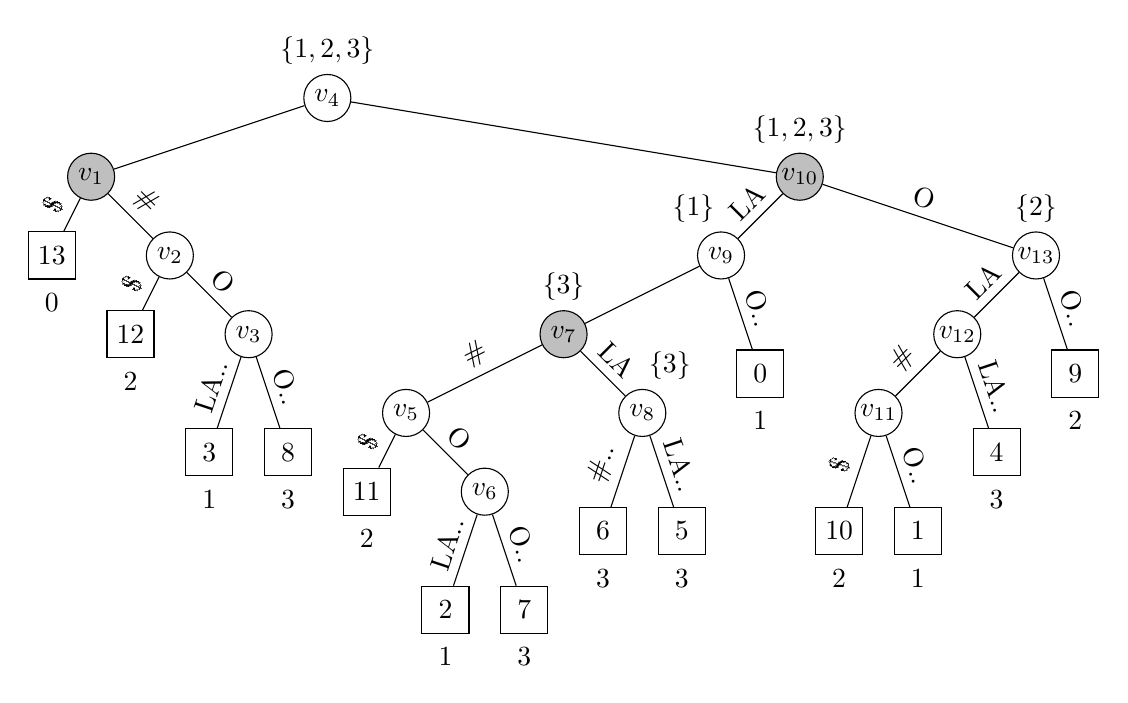
\begin{tikzpicture}[x={(5mm, 0mm)}]
  \tikzstyle{vertex}=[draw,minimum size=17pt, inner sep=0pt]
  \node[vertex, circle] (v4) at (0, 0) {$v_4$};
  \node (l4) at (0, 0.6) {$\{1,2,3\}$};

  \node[vertex, circle, fill=lightgray] (v1) at (-6, -1) {$v_1$};
  \draw (v4) -- (v1);

  \node[vertex, circle] (v2) at (-4, -2) {$v_2$};
  \draw (v1) -- (v2) node[above, sloped, pos=0.5] {\#};

  \node[vertex, circle] (v3) at (-2, -3) {$v_3$};
  \draw (v2) -- (v3) node[above, sloped, pos=0.5] {O};

  \node[vertex, circle, fill=lightgray] (v10) at (12, -1) {$v_{10}$};
  \node (l10) at (12, -0.4) {$\{1,2,3\}$};
  \draw (v4) -- (v10);

  \node[vertex, circle] (v9) at (10, -2) {$v_9$};
  \node (l9) at (9.3, -1.4) {$\{1\}$};
  \draw (v10) -- (v9) node[above, sloped, pos=0.5] {LA};

  \node[vertex, circle, fill=lightgray] (v7) at (6, -3) {$v_7$};
  \node (l7) at (6, -2.4) {$\{3\}$};
  \draw (v9) -- (v7);

  \node[vertex, circle] (v5) at (2, -4) {$v_5$};
  \draw (v7) -- (v5) node[above, sloped, pos=0.5] {\#};

  \node[vertex, circle] (v6) at (4, -5) {$v_6$};
  \draw (v5) -- (v6) node[above, sloped, pos=0.5] {O};

  \node[vertex, circle] (v8) at (8, -4) {$v_8$};
  \node (l8) at (8.7, -3.4) {$\{3\}$};
  \draw (v7) -- (v8) node[above, sloped, pos=0.5] {LA};

  \node[vertex, circle] (v13) at (18, -2) {$v_{13}$};
  \node (l13) at (18, -1.4) {$\{2\}$};
  \draw (v10) -- (v13) node[above, sloped, pos=0.5] {O};

  \node[vertex, circle] (v12) at (16, -3) {$v_{12}$};
  \draw (v13) -- (v12) node[above, sloped, pos=0.5] {LA};

  \node[vertex, circle] (v11) at (14, -4) {$v_{11}$};
  \draw (v12) -- (v11) node[above, sloped, pos=0.5] {\#};

  \node[vertex] (s13) at (-7, -2) {$13$};
  \node (d13) at (-7, -2.6) {$0$};
  \draw (v1) -- (s13) node[above, sloped, pos=0.5] {\$};

  \node[vertex] (s12) at (-5, -3) {$12$};
  \node (d12) at (-5, -3.6) {$2$};
  \draw (v2) -- (s12) node[above, sloped, pos=0.5] {\$};

  \node[vertex] (s3) at (-3, -4.5) {$3$};
  \node (d3) at (-3, -5.1) {$1$};
  \draw (v3) -- (s3) node[above, sloped, pos=0.5] {LA..};

  \node[vertex] (s8) at (-1, -4.5) {$8$};
  \node (d8) at (-1, -5.1) {$3$};
  \draw (v3) -- (s8) node[above, sloped, pos=0.5] {O..};

  \node[vertex] (s11) at (1, -5) {$11$};
  \node (d11) at (1, -5.6) {$2$};
  \draw (v5) -- (s11) node[above, sloped, pos=0.5] {\$};

  \node[vertex] (s2) at (3, -6.5) {$2$};
  \node (d2) at (3, -7.1) {$1$};
  \draw (v6) -- (s2) node[above, sloped, pos=0.5] {LA..};

  \node[vertex] (s7) at (5, -6.5) {$7$};
  \node (d7) at (5, -7.1) {$3$};
  \draw (v6) -- (s7) node[above, sloped, pos=0.5] {O..};

  \node[vertex] (s6) at (7, -5.5) {$6$};
  \node (d6) at (7, -6.1) {$3$};
  \draw (v8) -- (s6) node[above, sloped, pos=0.5] {\#..};

  \node[vertex] (s5) at (9, -5.5) {$5$};
  \node (d5) at (9, -6.1) {$3$};
  \draw (v8) -- (s5) node[above, sloped, pos=0.5] {LA..};

  \node[vertex] (s0) at (11, -3.5) {$0$};
  \node (d0) at (11, -4.1) {$1$};
  \draw (v9) -- (s0) node[above, sloped, pos=0.5] {O..};

  \node[vertex] (s9) at (19, -3.5) {$9$};
  \node (d9) at (19, -4.1) {$2$};
  \draw (v13) -- (s9) node[above, sloped, pos=0.5] {O..};

  \node[vertex] (s4) at (17, -4.5) {$4$};
  \node (d4) at (17, -5.1) {$3$};
  \draw (v12) -- (s4) node[above, sloped, pos=0.5] {LA..};

  \node[vertex] (s10) at (13, -5.5) {$10$};
  \node (d10) at (13, -6.1) {$2$};
  \draw (v11) -- (s10) node[above, sloped, pos=0.5] {\$};

  \node[vertex] (s1) at (15, -5.5) {$1$};
  \node (d1) at (15, -6.1) {$1$};
  \draw (v11) -- (s1) node[above, sloped, pos=0.5] {O..};
\end{tikzpicture}

  \caption{The binary generalized suffix tree of an example document collection $\mathcal{D} = \texttt{LA O LA \# O LA LA LA \# O O LA \# \$}$. The filled vertices are the dummy nodes added to get a binary tree. Round nodes are inner nodes, square nodes are leaves corresponding to suffixes. The number below each leaf is the entry in the document array.}
  \label{fig:binaryGeneralizedSuffixTreeExample}
\end{figure}

\begin{algorithm}[htb]
  \begin{codebox}
    \Procname{$\proc{Document-Frequency}(q)$}
    \li $[l,r] \gets \proc{Backward-Search(\id{CSA}, q)}$
    \li $s \gets r - l + 1$
    \li $y \gets \proc{Select}_1(r, H)$
    \li \If $l \isequal 0$
        \Then
    \li   \Return $s - (y - r + 1)$
    \li \Else
    \li   $x \gets \proc{Select}_1(l, H)$
    \li   \Return $s - (y - r + 1 - (x - l + 1))$
        \End
  \end{codebox}
  \caption{Compute the document frequency $F_{\mathcal{D},q}$ for query $q$.}
  \label{alg:documentFrequency}
\end{algorithm}

\begin{Example}
  Figure~\ref{fig:binaryGeneralizedSuffixTreeExample} shows the \id{BGST} for \texttt{LA O LA \# O LA LA LA \# O O LA \# \$}. We get the following bitvector $H$:
  \begin{align*}
    H = 1
    \underbrace{1}_{v_1}
    \underbrace{1}_{v_2}
    \underbrace{1}_{v_3}
    \underbrace{0001}_{v_4}
    \underbrace{1}_{v_5}
    \underbrace{1}_{v_6}
    \underbrace{01}_{v_7}
    \underbrace{01}_{v_8}
    \underbrace{01}_{v_9}
    \underbrace{0001}_{v_{10}}
    \underbrace{1}_{v_{11}}
    \underbrace{1}_{v_{12}}
    \underbrace{01}_{v_{13}}
  \end{align*}
  Let's now consider $q = \texttt{LA}$. Then \proc{Backward-Search} returns suffix array interval $[4,9]$. Executing the steps in Algorithm~\ref{alg:documentFrequency} yields $s = 6$, $y = 15$ and $x = 7$, so that $3$ is returned.
\end{Example}

\begin{Theorem}
  The document frequency can be calculated with an index needing $\mathcal{O}(n + \vert \id{CSA} \vert)$ bits space.
\end{Theorem}

\begin{Proof}
  The bitvector $H$ has maximum size $2n - N$. Additionally $o(n)$ bits for a constant time select structure are needed. The only thing left is the space needed for \id{CSA}.
\end{Proof}

\subsection{Calculating $F_{\mathcal{D}_v, q}$}

Let $F_{\mathcal{D}_v, q}$ be the subset of documents which are represented by a node in the wavelet tree over the document array. To compute it efficiently we introduce another array:

\begin{Definition}
  The \defi{repetition array}{Repetition Array} $R$ contains for each $0$ in $H$ the corresponding repeated element of the associated node.
\end{Definition}

We can build a wavelet tree \id{WTD} over the document array and a wavelet tree \id{WTR} over the repetition array. Using $\proc{Select}_1$ we can as above convert an interval $[l,r]$ of the suffix array into ranges in the two wavelet trees. When traversing \id{WTD} we can simultaneously traverse \id{WTR}. The size of the range in \id{WTR} always counts the number of repetitions.

\begin{Example}
  Continuing above example, we get for $H$ and $R$:
  \begin{align*}
    H &= 1
    \underbrace{1}_{v_1}
    \underbrace{1}_{v_2}
    \underbrace{1}_{v_3}
    \underbrace{0001}_{v_4}
    \underbrace{1}_{v_5}
    \underbrace{1}_{v_6}
    \underbrace{01}_{v_7}
    \underbrace{01}_{v_8}
    \underbrace{01}_{v_9}
    \underbrace{0001}_{v_{10}}
    \underbrace{1}_{v_{11}}
    \underbrace{1}_{v_{12}}
    \underbrace{01}_{v_{13}} \\
    R &=
    \underbrace{123}_{v_4}
    \underbrace{3}_{v_2}
    \underbrace{3}_{v_8}
    \underbrace{1}_{v_9}
    \underbrace{123}_{v_{10}}
    \underbrace{2}_{v_{13}}
  \end{align*}
\end{Example}


  \printindex
  \printbibliography
\end{document}
